\FloatBarrier
\section{CP violation sensitivity}
\label{sec:cp_sens}

In this section, CPV sensitivity results are presented. For simplicity, only true NO will be shown unless explicitly stated. In all cases, a joint ND+FD fit is performed, and a $\theta_{13}$ penalty is always applied to incorporate the reactor measurement, as described in Section~\ref{sec:analysis_framework}. An equal split between FHC and RHC running is assumed based on the results obtained in Section~\ref{sec:run_plan_opt}. Asimov sensitivities, as shown in Section~\ref{sec:run_plan_opt}, are instructive but do not give information on how the expected sensitivity may vary with statistical or systematic uncertainties, or for variations in the other oscillation parameters of interest.

\begin{figure}[htbp]
  \centering
  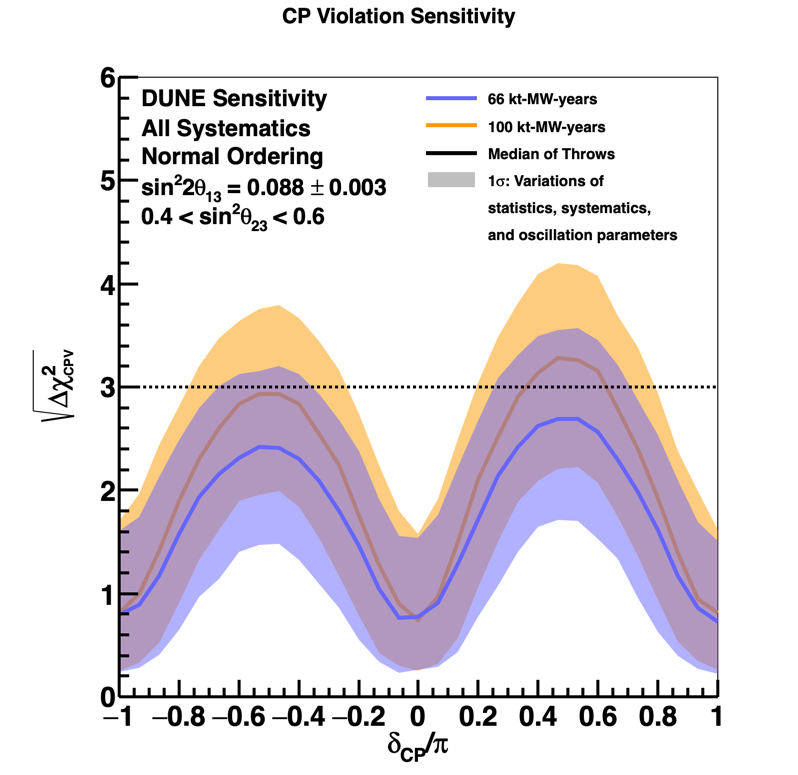
\includegraphics[width=1\linewidth, trim={0cm 0cm 0cm 2.3cm}, clip]{cpv_two_exps_throws_nh_2019_v4_lowexp.png}\\
  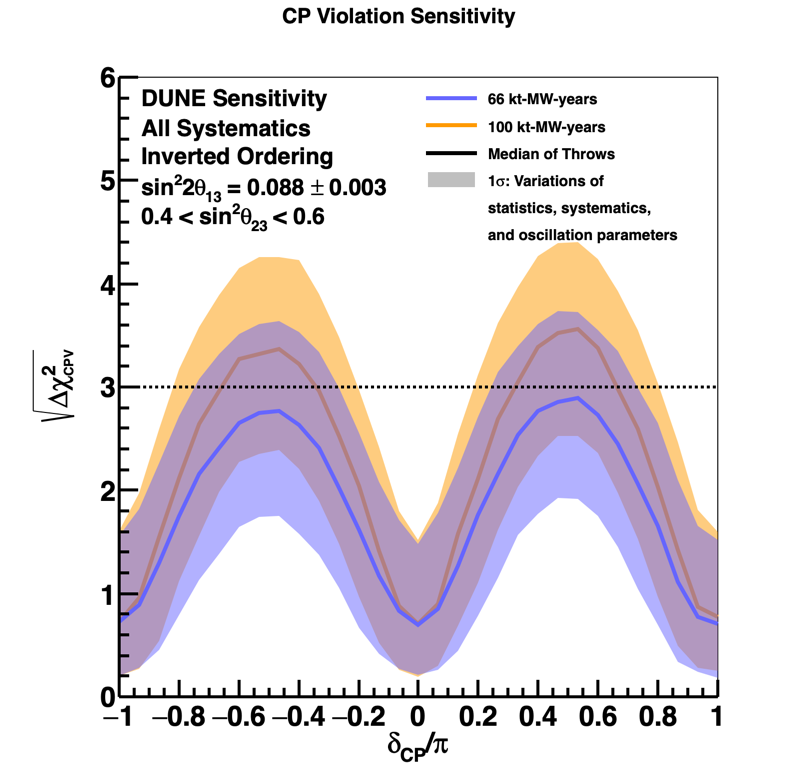
\includegraphics[width=1\linewidth, trim={0cm 0cm 0cm 2.3cm}, clip]{cpv_two_exps_throws_ih_2019_v4_lowexp.png}
  \caption{Significance of the DUNE determination of CP-violation ($\deltacp \neq \{0,\pm\pi\}$) as a function of the true value of \deltacp, for 66 kt-MW-yr (blue) and 100 kt-MW-yr (orange) exposures, for normal (top) and inverted (bottom) orderings. The width of the transparent bands cover 68\% of fits in which random throws are used to simulate systematic, oscillation parameter and statistical variations, with independent fits performed for each throw constrained by prior uncertainties. The solid lines show the median significance.}
  \label{fig:cpv_bands}
\end{figure}
Figure~\ref{fig:cpv_bands} shows the significance with which CPV ($\deltacp \neq \{0,\pm\pi\}$) can be observed for both NO and IO, for exposures of 66 and 100 kt-MW-yr.  The sensitivity metric used is the square root of the difference between the best fit $\chi^{2}$ values obtained for a CP-conserving fit and one where \deltacp is allowed to vary, as shown in Equation~\ref{eq:cpv_chi2}, which is calculated for each throw of the systematic, other oscillation parameters and statistics. %This constant-\dchisq method is valid as long as Wilks' theorem can be applied~\cite{wilks}.

The sensitivity shown in Figure~\ref{fig:cpv_bands} has a characteristic double peak structure because the significance of a CPV measurement decreases around CP-conserving values. The systematic and statistical variations mean that all throws have $\dchisqCPV \geq 0$, and therefore neither the median significance nor the band showing the central 68\% of throws reach exactly 0 at CP-conserving values. This is entirely expected, it simply means that random variations in the data will cause us to obtain a 1$\sigma$ measurement of CPV $\sim$32\% of the time for CP-conserving values. Median significances are slightly higher for IO than for NO, and by exposures of 100 kt-MW-yr, the median significance exceeds 3$\sigma$ for the maximal CP-violating values of $\pm\pi/2$. This presentation of the CPV sensitivity was followed in Ref.~\cite{Abi:2020qib}, and is very informative at high exposures. Around CP-conserving values ($\deltacp = \{0,\pm\pi\}$), the distribution of the sensitivity metric $\sqrt{\dchisqCPV}$ is non-Gaussian for all exposures. Additionally, at lower exposures, as shown in Figure~\ref{fig:cpv_bands}, the distribution of $\sqrt{\dchisqCPV}$ around maximally CP-violating values of $\deltacp = \pm\pi/2$ is increasingly non-Gaussian, making the spread in sensitivity harder to interpret with this presentation.

% \FloatBarrier
% \subsection{Feldman-Cousins studies}
The CPV significance in Figure~\ref{fig:cpv_bands} (and previously in Ref.~\cite{Abi:2020qib}) is calculated using constant \dchisq critical values, where $\dchisqCPV \leq 1, 4, 9$ corresponds to a significance of 1, 2 and 3$\sigma$ for one degree of freedom. This assumption holds when Wilks' theorem can be applied~\cite{wilks}, but can lead to incorrect coverage where it cannot. It is known to break down for low-statistics samples, around physical boundaries, in the case of cyclic parameters, and where there are significant degeneracies. It is likely that a constant \dchisq treatment will break down for \deltacp, where all of these issues apply, as has indeed been shown by the T2K Collaboration~\cite{Abe:2021gky}.

The Feldman-Cousins method~\cite{Feldman:1997qc} is a brute force numerical method to calculate confidence intervals with correct coverage. A large number of toy experiments are produced, where the parameter(s) of interest (here \deltacp) is set to a desired true value, all other systematic and oscillation parameters are thrown, as described in Section~\ref{sec:analysis_framework}, and a statistical throw is made, for the two ND samples and four FD sample used in the analysis. Then two fits are performed, one where the parameter(s) of interest are fixed to the true value, and another where the test statistic is minimized with respect to the parameter(s) of interest. In both fits, all other parameters are allowed to vary. For each throw, the profile likelihood ratio \dchisqFC is calculated using the minimum $\chi^{2}$ values for those two fits, as in Equation~\ref{eq:dchisq_fc}.
\begin{linenomath*}
  \begin{equation}
    \dchisqFC = \chi^{2}(\theta_{\mathrm{true}}) - \min_{\theta}\chi^{2}(\theta)
    \label{eq:dchisq_fc}
  \end{equation}
\end{linenomath*}
\begin{figure}[htbp]
  \centering
  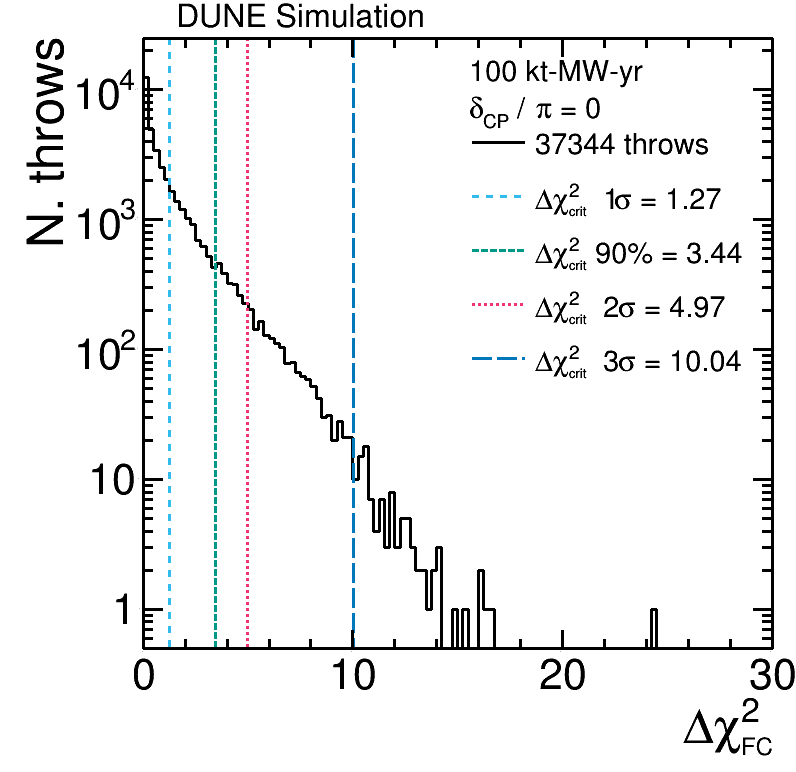
\includegraphics[width=0.8\columnwidth]{nh_FC_ndfd_100ktMWyr_dcp0.png}
  \caption{Distribution of \dchisqFC values, calculated using Equation~\ref{eq:dchisq_fc}, for a large number of throws with true $\deltacp = 0$, and a 100 kt-MW-yr exposure. The \dchisqcrit values (vertical lines) obtained using the Feldman-Cousins method show the \dchisqFC value below which 68.27\% (1$\sigma$), 90\%, 95.45\% (2$\sigma$) and 99.73\% (3$\sigma$) of throws reside, with the calculated values given in the legend. The number of throws used is also given.}
  \label{fig:fc_throws}
\end{figure}
The distribution of these throws is used to calculate the \dchisqFC value that gives the desired coverage, with the appropriate fraction of toys above/below the calculated value. These are labelled {\it critical values}, and are denoted \dchisqcrit. A distribution of \dchisqFC values is shown in Figure~\ref{fig:fc_throws} for an example ND+FD analysis with a 100kt-MW-yr exposure at the far detector, equal FHC and RHC run fractions, and the reactor $\theta_{13}$ constraint applied. In Figure~\ref{fig:fc_throws}, the \dchisqcrit values corresponding to for 68.27\% (1$\sigma$), 90\%, 95.45\% (2$\sigma$) and 99.73\% (3$\sigma$) of the throws are indicated. The \dchisqcrit values were only calculated up to the 3$\sigma$ level due to the very large number of throws required for higher confidence levels.

An uncertainty on the value of \dchisqcrit obtained from the toy throw distribution (e.g., Figure~\ref{fig:fc_throws}), is obtained using a bootstrap rethrowing method~\cite{rice2006mathematical}. The empirical PDF obtained from the throws is treated as the true PDF, and $B$ independent samples of size $n$ are drawn from it, where $n$ is the total number of throws used to build the empirical PDF. Note that each throw can be drawn multiple times in this method, so the ensemble of throws is different in each sample. Then, the standard deviation $s_{\hat{\vartheta}}$, on the \dchisqcrit values of interest, $\vartheta$, are calculated for each of the $B$ samples using:
\begin{linenomath*}
\begin{equation}
  s_{\hat{\vartheta}} = \sqrt{\frac{1}{B-1} \sum^{B}_{i=0} (\vartheta_{i}^{*} - \bar{\vartheta}^{*})^{2}},
  \label{eq:fc_uncertainty}
\end{equation}
\end{linenomath*}
where $\vartheta_{i}^{*}$ denotes the calculated \dchisqcrit value of interest for each of the samples, and $\bar{\vartheta}^{*}$ is their average value.

\begin{figure}[htbp]
  \centering
  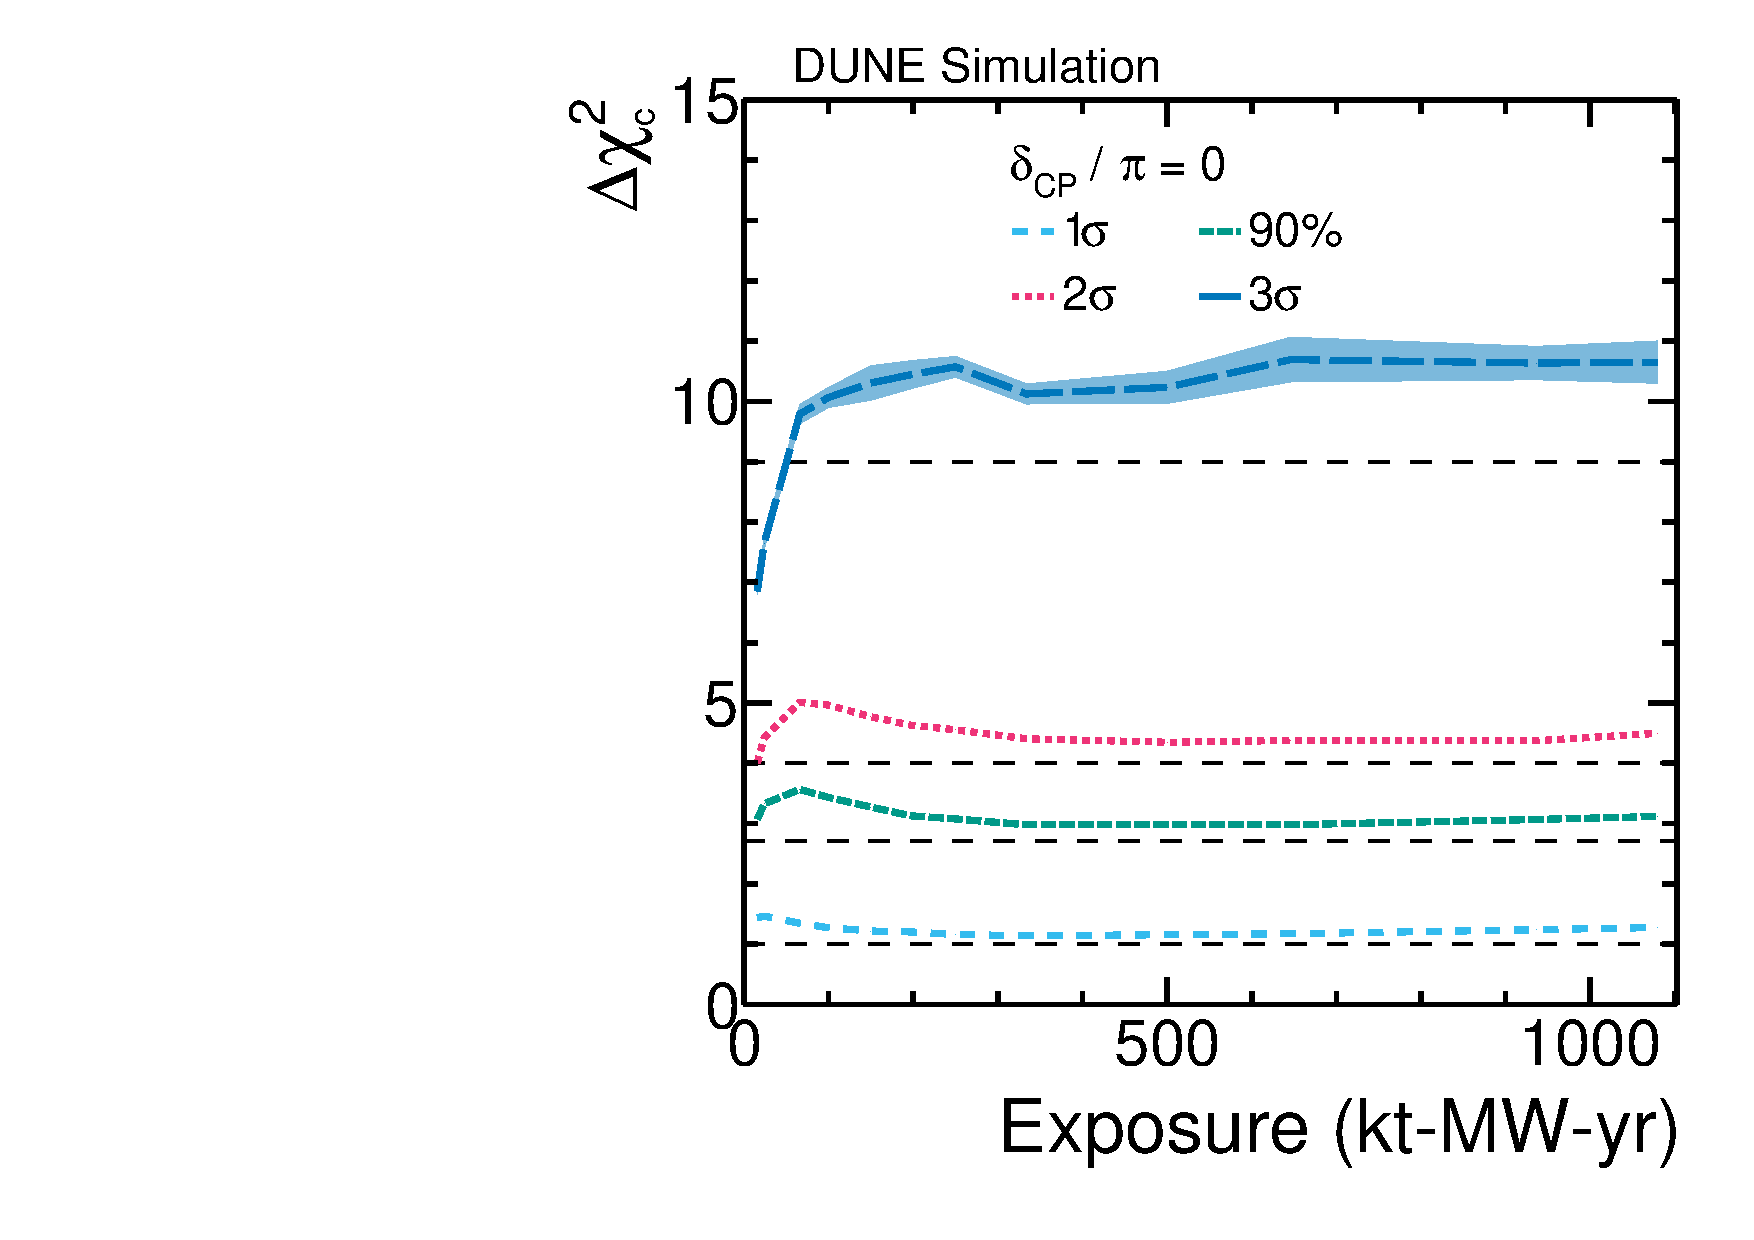
\includegraphics[width=0.8\columnwidth]{dchi2crit_vs_exp_dcp0.pdf}
  \caption{The \dchisqcrit values corresponding to 68.27\% (1$\sigma$), 90\%, 95.45\% (2$\sigma$) and 99.73\% (3$\sigma$) of throws, shown for true $\deltacp = 0$, as a function of exposure. A linear $x$-axis scale is used to highlight the stability of \dchisqcrit values for large exposures. The uncertainty on the \dchisqcrit values is obtained using Equation~\ref{eq:fc_uncertainty}, and is indicated as the shaded line. To guide the eye, horizontal dashed lines are included which indicate the 1$\sigma$, 90\%, 2$\sigma$ and 3$\sigma$ \dchisq values assumed using the constant-\dchisq method, with one degree of freedom. The distribution of throws used produced to calculate the \dchisqcrit values shown are given in Figure~\ref{fig:fc_throws_exp}.}
  \label{fig:fc_vs_exp}
\end{figure}
Figure~\ref{fig:fc_vs_exp} shows the evolution of the \dchisqcrit values as a function of exposure for $\deltacp = 0$, the relevant value for CPV sensitivity, for an ND+FD analysis with equal FHC and RHC running and the reactor $\theta_{13}$ constraint applied.
%Several values were checked for $\deltacp = \pm\pi$ and similar results were found, so Figure~\ref{fig:fc_vs_exp} can be thought of as the threshold for CPV significance.
For all significance levels tested, the \dchisqcrit rise quickly as a function of exposure, and stabilize at values slightly higher than those suggested by the constant \dchisq method by exposures of $\sim$100 kt-MW-yr. The initial rise in the \dchisqcrit values is due to the low statistics at those exposures. Overall, this implies that the CPV significance is slightly weaker than what would be inferred from $\sigma = \sqrt{\dchisqCPV}$, as used for example in Figure~\ref{fig:cpv_bands}. Crucially, there is no constant increase in the \dchisqcrit values over time as has been reported by the T2K Collaboration~\cite{Abe:2021gky}. Details on the number of toy throws used at each point of Figure~\ref{fig:fc_vs_exp} are given in the Appendix, and the toy throw distributions from which the \dchisqcrit values and their uncertainties were calculated are shown in Figure~\ref{fig:fc_throws_exp}.

\begin{figure}[htbp]
  \centering
  \subfloat[100 kt-MW-yr]  {\label{fig:fc_vs_dcp_100}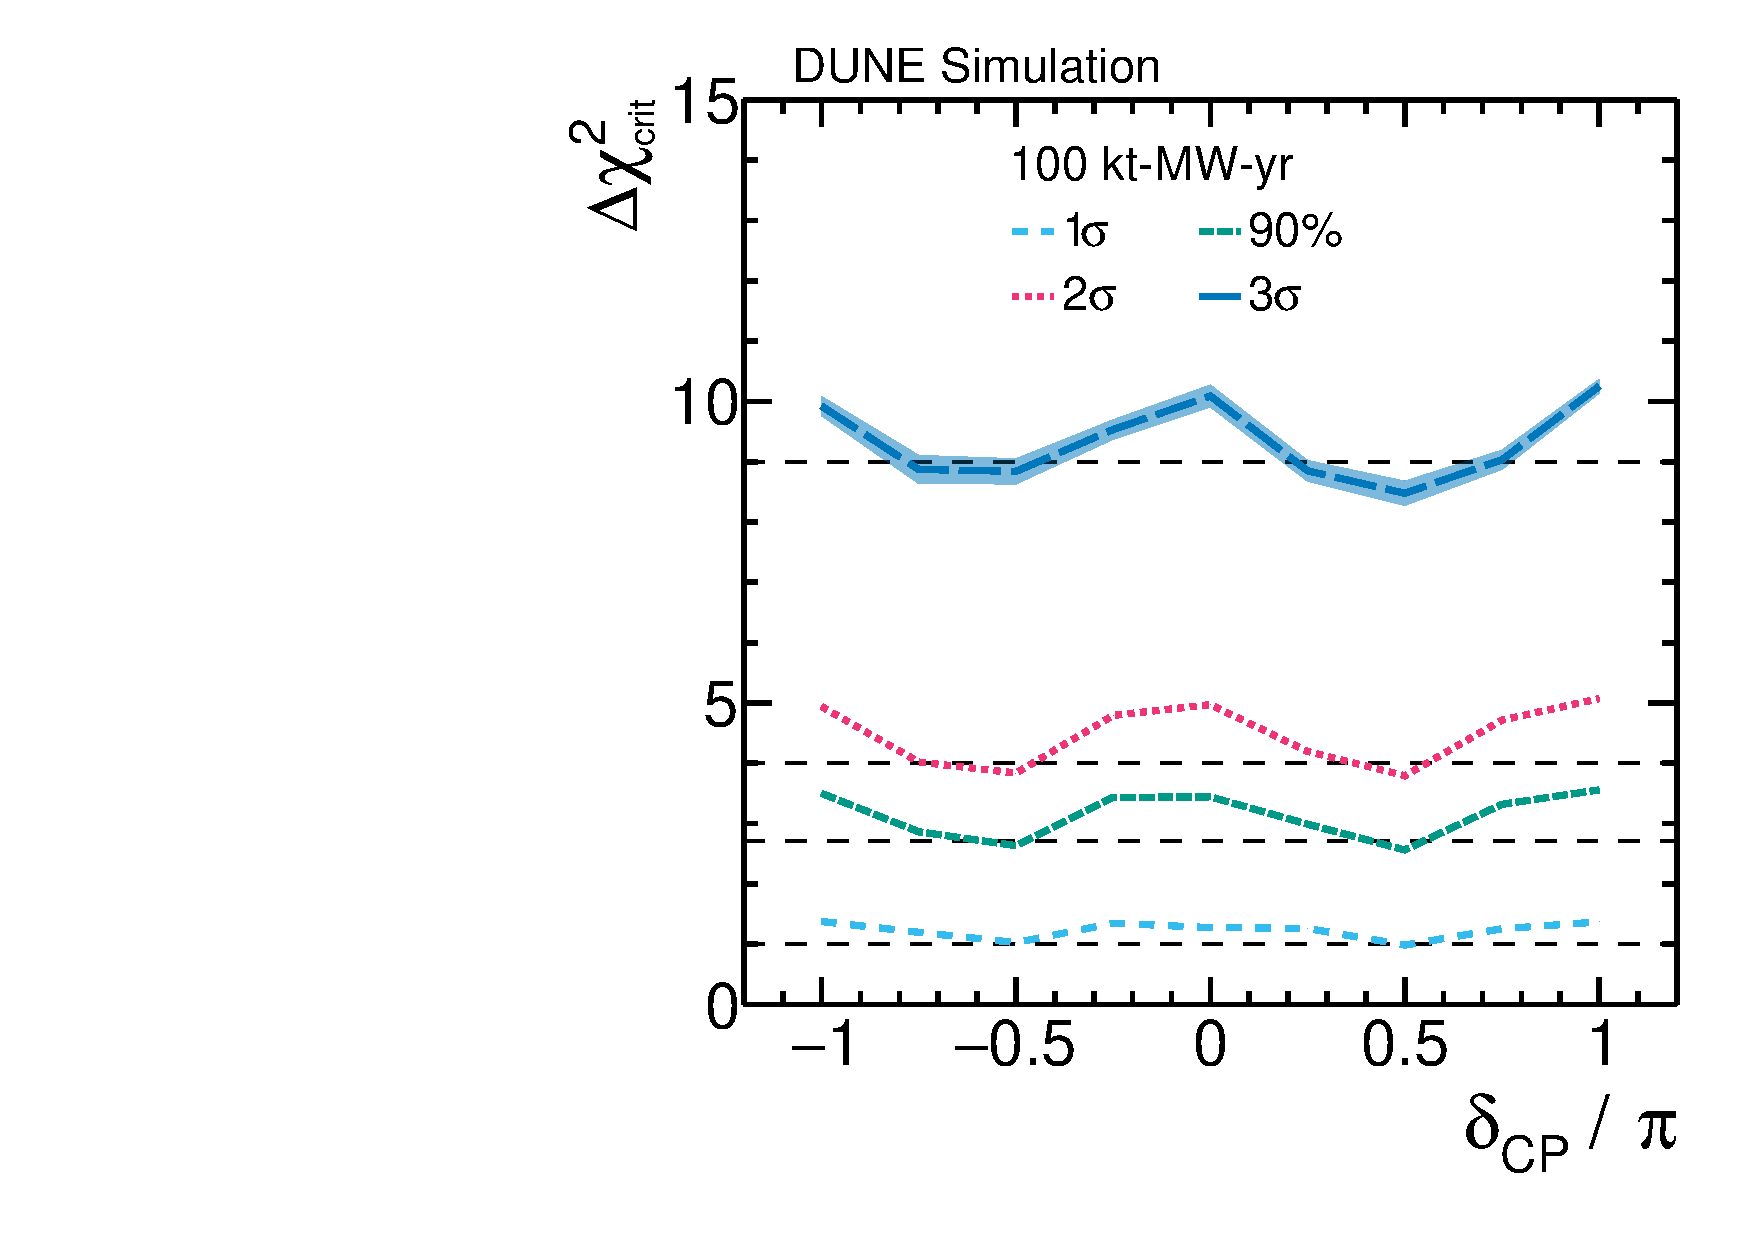
\includegraphics[width=0.8\columnwidth]{dchi2crit_vs_dcp_100ktMWyr.pdf}}\\
  \subfloat[334 kt-MW-yr]  {\label{fig:fc_vs_dcp_334}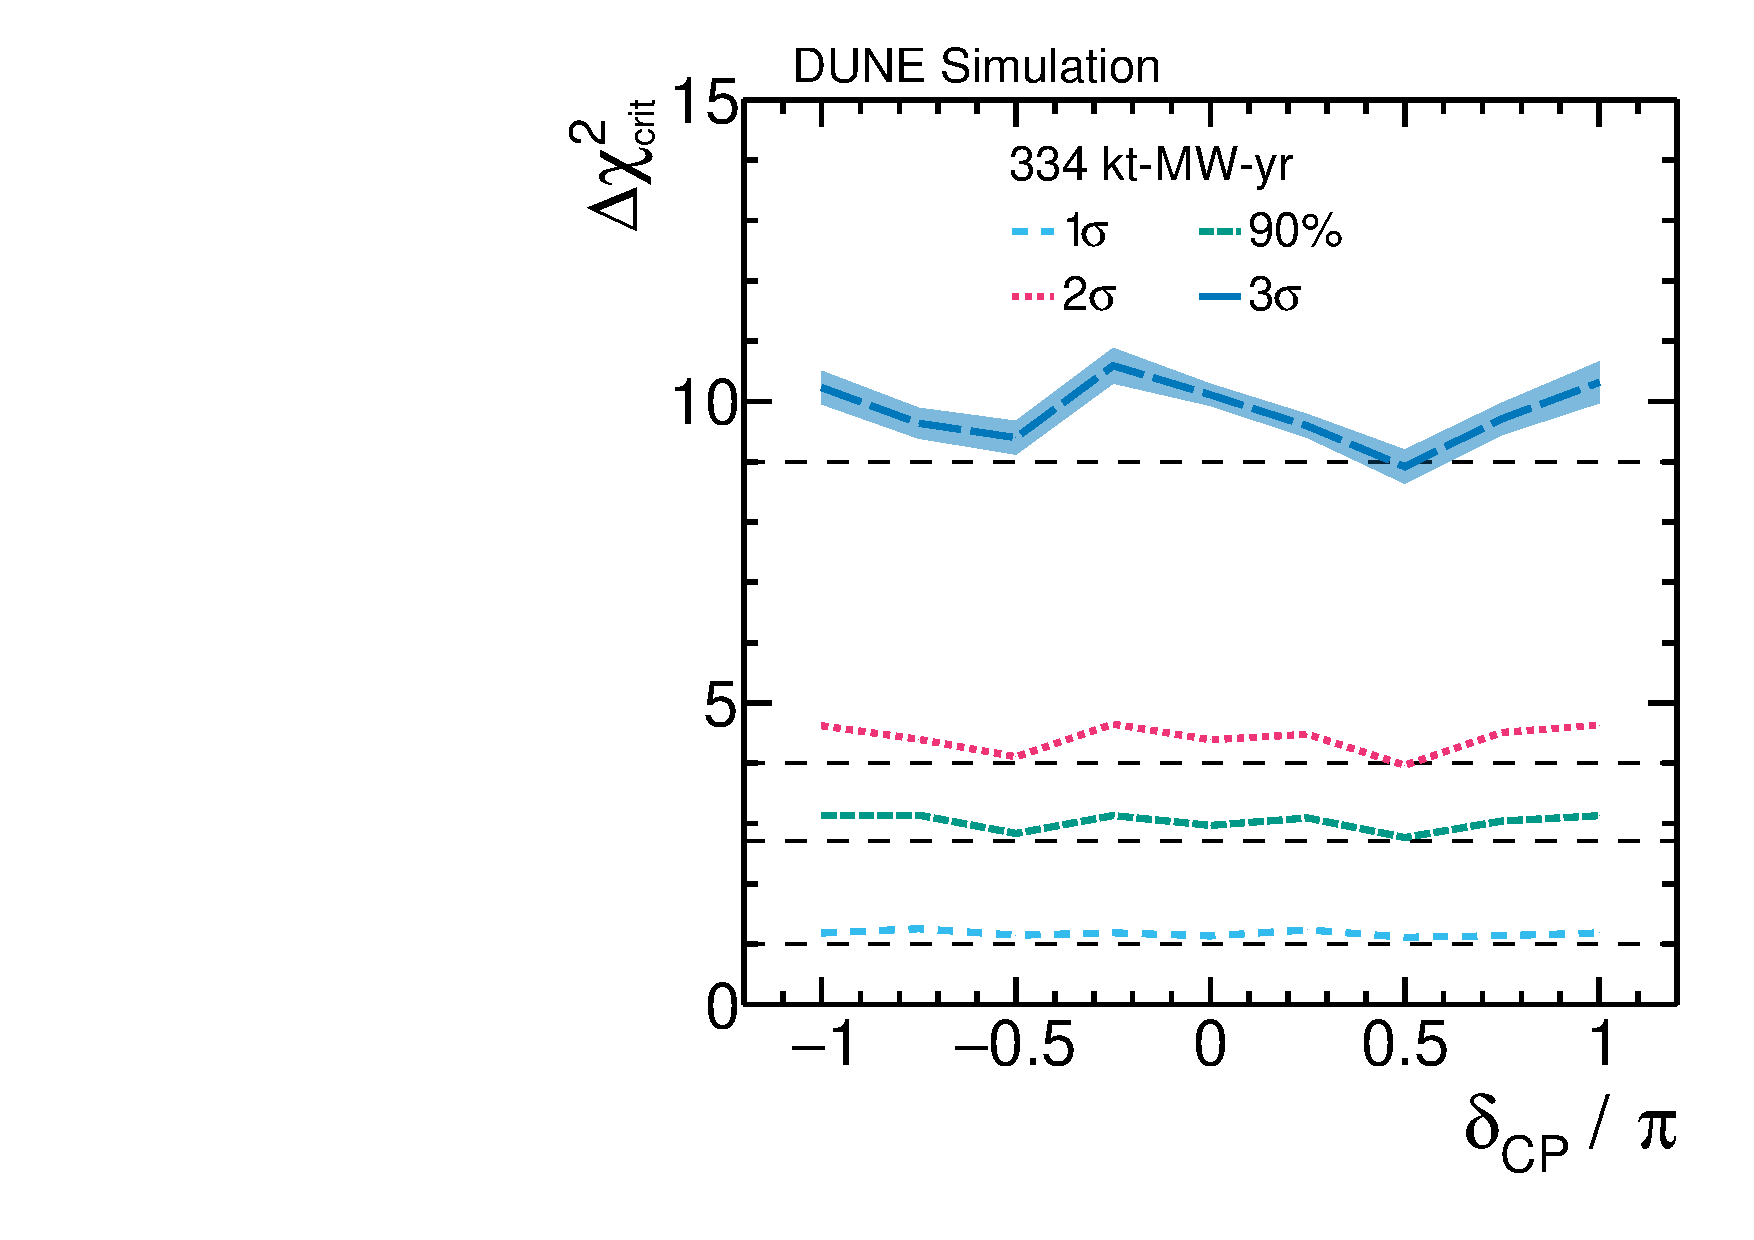
\includegraphics[width=0.8\columnwidth]{dchi2crit_vs_dcp_334ktMWyr.pdf}}
  \caption{The \dchisqcrit values corresponding to 68.27\% (1$\sigma$), 90\%, 95.45\% (2$\sigma$) and 99.73\% (3$\sigma$) of throws, shown as a function of true \deltacp, for exposures of 100 kt-MW-yr and 334 kt-MW-yr. The uncertainty on the \dchisqcrit values is obtained using Equation~\ref{eq:fc_uncertainty}, and is indicated as the shaded line. To guide the eye, horizontal dashed lines are included which indicate the 1$\sigma$, 90\%, 2$\sigma$ and 3$\sigma$ \dchisqCPV values assumed using the constant-\dchisq method, with one degree of freedom. The distribution of throws used produced to calculate the \dchisqcrit values shown are given in Figure~\ref{fig:fc_throws_100kt-MW-yr} (Figure~\ref{fig:fc_throws_334kt-MW-yr}) for 100 kt-MW-yr (334 kt-MW-yr).}
  \label{fig:fc_vs_dcp}
\end{figure}
As \deltacp is a cyclical parameter, with physical boundaries at $\pm\pi$, it is interesting to see how the \dchisqcrit values evolve as a function of it. Figure~\ref{fig:fc_vs_dcp} shows the \dchisqcrit as a function of true \deltacp, for an ND+FD analysis with equal FHC and RHC running including the reactor $\theta_{13}$ constraint, for both 100 kt-MW-yr and 334 kt-MW-yr exposures. There is a noticeable, although not large, depression in the \dchisqcrit values at $\deltacp = \pm\pi/2$ for all significance levels considered. This effect is larger at the lower, 100 kt-MW-yr, exposure, and is larger at higher significance levels. It is also clear from Figure~\ref{fig:fc_vs_dcp} that the \dchisqcrit behaviour is very similar at $\deltacp = \pm\pi/2$ as at $\deltacp = 0$. Although the \dchisqcrit values are relevant for CPV sensitivity, this evolution of the \dchisqcrit values with \deltacp will be important for estimating DUNE's \deltacp resolution. Details on the number of toy throws used at each point of Figure~\ref{fig:fc_vs_dcp} are given in the Appendix, and the toy throw distributions used to calculate the \dchisqcrit values and uncertainties are shown for the 100 kt-MW-yr (334 kt-MW-yr) test points in Figure~\ref{fig:fc_throws_100kt-MW-yr} (Figure~\ref{fig:fc_throws_334kt-MW-yr}).

\begin{figure*}[htbp]
  \centering
  \captionsetup[subfloat]{captionskip=-4pt}
  \subfloat[24 kt-MW-yr]  {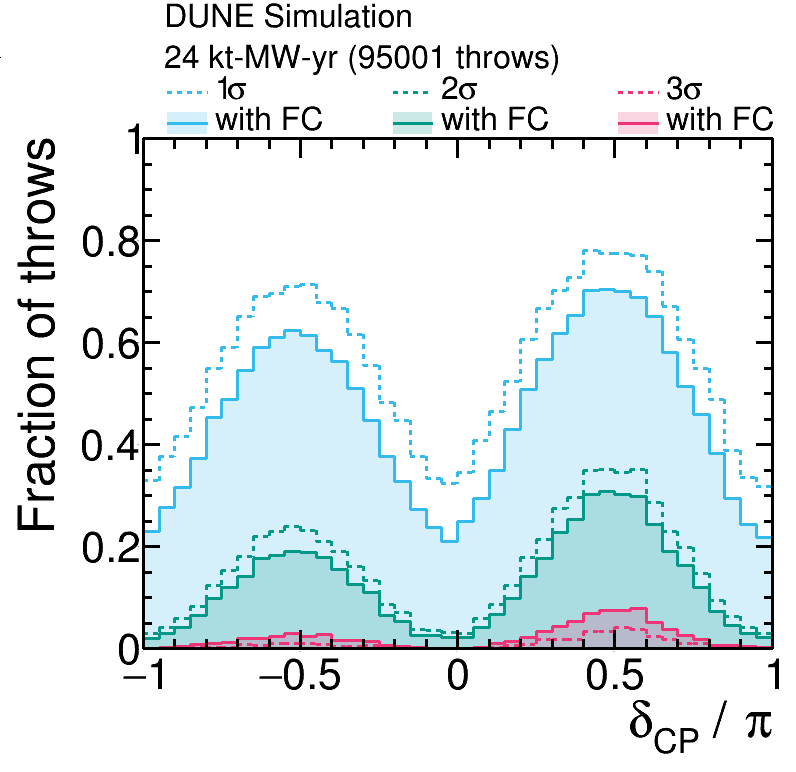
\includegraphics[width=0.33\linewidth]{cpv_throws_withFC_24ktMWyr_NH_th13.png}}
  \subfloat[66 kt-MW-yr]  {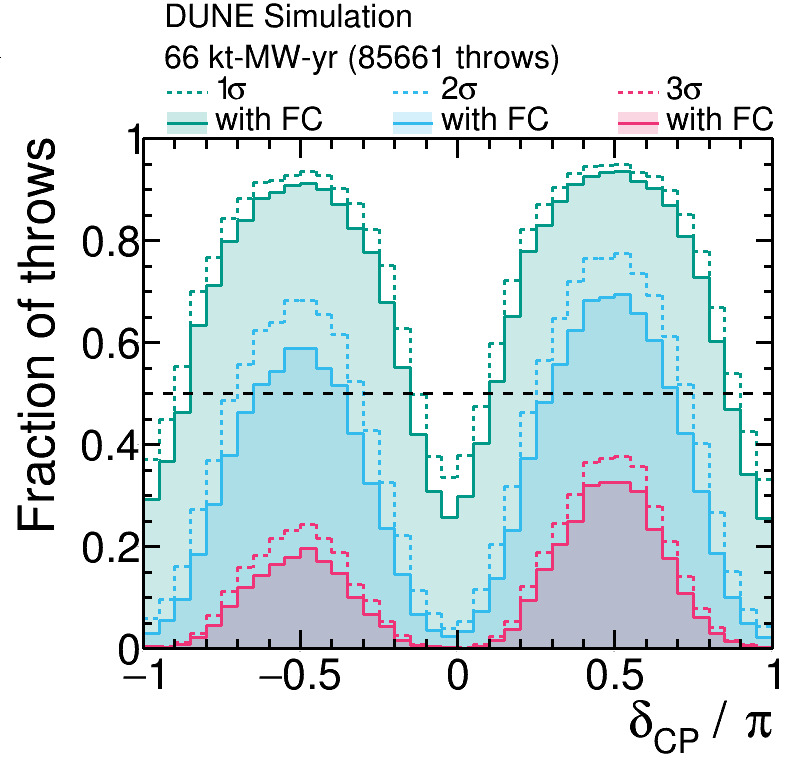
\includegraphics[width=0.33\linewidth]{cpv_throws_withFC_66ktMWyr_NH_th13.png}}
  \subfloat[100 kt-MW-yr] {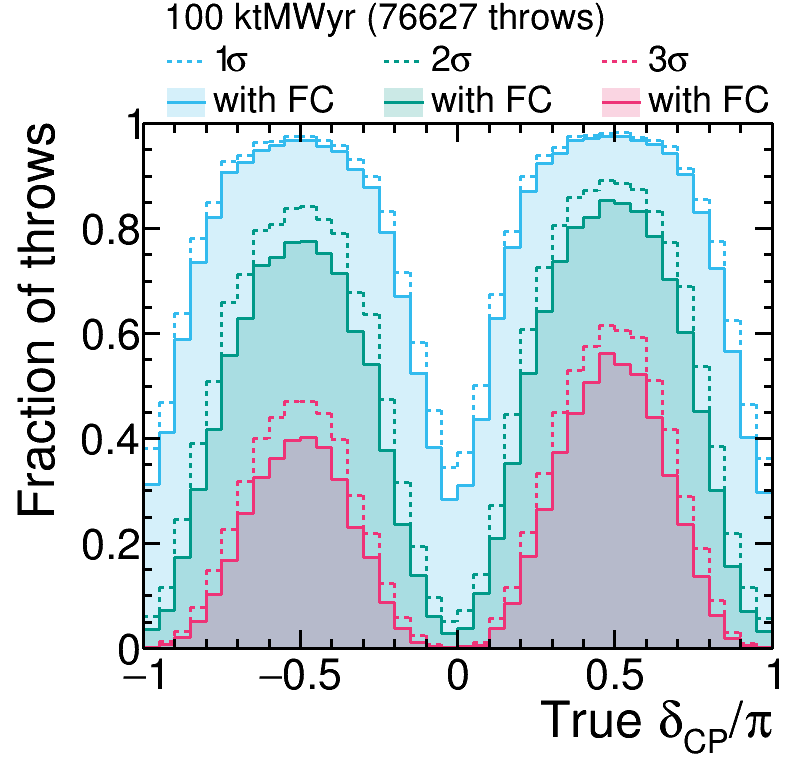
\includegraphics[width=0.33\linewidth]{cpv_throws_withFC_100ktMWyr_NH_th13.png}}\\
  \subfloat[150 kt-MW-yr] {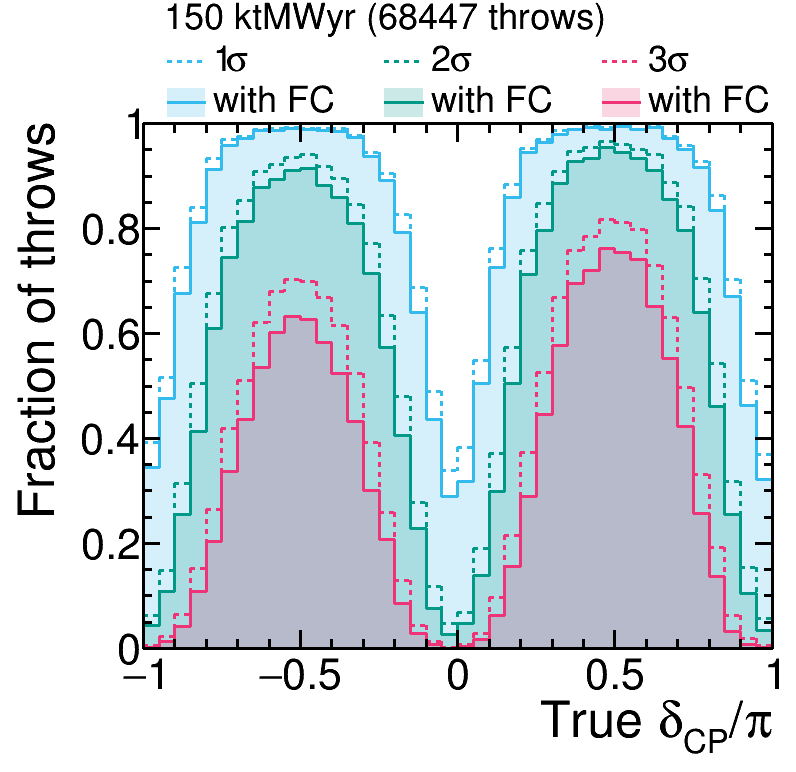
\includegraphics[width=0.33\linewidth]{cpv_throws_withFC_150ktMWyr_NH_th13.png}}
  \subfloat[197 kt-MW-yr] {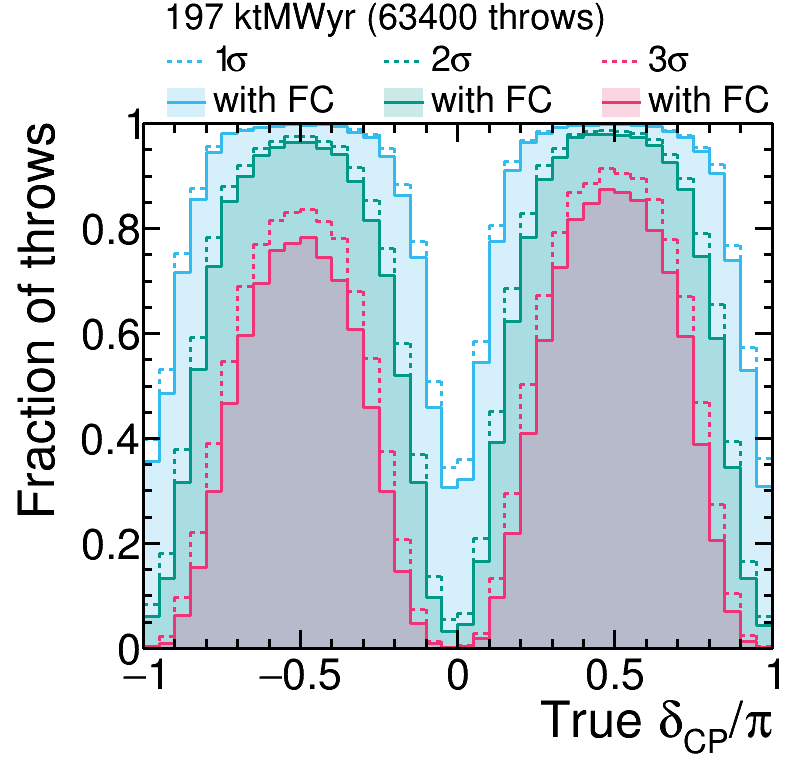
\includegraphics[width=0.33\linewidth]{cpv_throws_withFC_197ktMWyr_NH_th13.png}}
  \subfloat[334 kt-MW-yr] {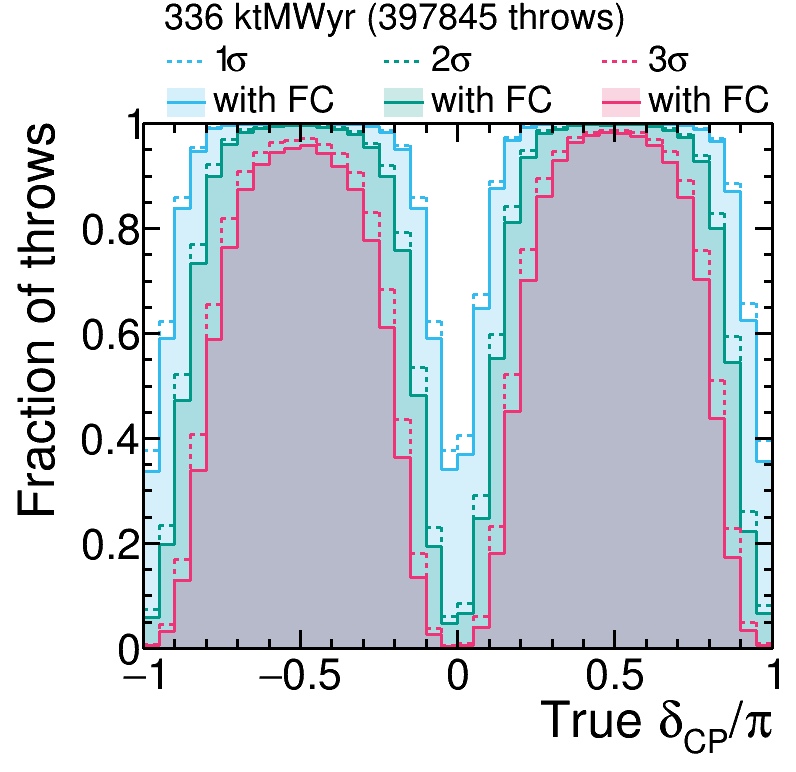
\includegraphics[width=0.33\linewidth]{cpv_throws_withFC_334ktMWyr_NH_th13.png}}
  \caption{Fraction of throws for which significance of DUNE's CP-violation test ($\deltacp \neq \{0,\pm\pi\}$) exceeds 1--3$\sigma$, calculated using both the FC (shaded histograms) and constant-\dchisq (dashed lines) methods, as a function of the true value of \deltacp. Shown for NO, for a number of different exposures. The number of throws used to make each figure is also shown.}
  \label{fig:cpv_over_time_fc}
\end{figure*}
DUNE's CPV sensitivity is calculated using Equation~\ref{eq:cpv_chi2} from an ensemble of throws of all systematic, other oscillation parameters and statistics. Figure~\ref{fig:cpv_over_time_fc} shows the fraction of throws for which DUNE would observe a CPV significance above a discrete threshold, as a function of the true value of \deltacp, for 1--3$\sigma$ significances and for a variety of exposures. The shaded histograms show the complete treatment including FC, while the dashed histograms show the constant-\dchisq treatment, to show the deviation from Wilks' theorem, and to facilitate comparison at higher significances where the FC treatment becomes computationally prohibitive.

The point at which the median significance (50\% of throws) passes different significance thresholds can be easily read from the figures, and can be compared with those shown in Figure~\ref{fig:cpv_bands}. The same double peak structure seen in Figure~\ref{fig:cpv_bands} can be observed. The median significance for measuring CPV exceeds 3$\sigma$ after $\sim$100 kt-MW-yr, but a significant fraction of throws exceed 3$\sigma$ at shorter exposures. By 334 kt-MW-yr exposures, the fraction of throws for which the significance is less than 3$\sigma$ at maximal values of \deltacp is very small. In general, the effect of the Feldman-Cousins correction is to reduce the fraction of toy throws that cross each significance threshold (with respect to the constant-\dchisq result), by a maximum of $\sim$10\%, but the exact fraction changes as a function of true \deltacp value and exposure. An exception to this general trend is the 3$\sigma$ behaviour at 24 kt-MW-yr, the lowest exposure shown, where the significance increases. This is due to fall in the 3$\sigma$ \dchisqcrit value towards the lowest exposures observed in Figure~\ref{fig:fc_vs_exp}. The number of throws carried out at each exposure is indicated on each plot. The number of throws decreases as a function of exposure because fixed computing resources were used for each configuration, and the time for the ensemble of fits carried out for each throw to complete increases slightly with exposure. The final 334 kt-MW-yr exposure has more throws because it was generated for the analysis presented in Ref.~\cite{Abi:2020qib}, where more than one projection was considered --- requiring more throws to sample the space.
\begin{figure*}[htbp]
  \centering
  \subfloat[$\deltacp = -\pi/2$] {\includegraphics[width=0.8\columnwidth]{{fraction_throws_vs_exp_dcp-0.5_FC}.pdf}}
  \subfloat[50\% of \deltacp values] {\includegraphics[width=0.8\columnwidth]{{fraction_throws_vs_exp_dcprange_0.5_FC}.pdf}}
\caption{Fraction of throws for which the significance of DUNE's CP-violation test ($\deltacp \neq \{0,\pm\pi\}$) exceeds 1--3$\sigma$, for $\deltacp = -\pi/2$ and for 50\% of \deltacp values, calculated with the FC (solid lines) and constant-\dchisq (dashed lines) methods, as a function of exposure.}
  \label{fig:cpv_vs_exp_fc}
\end{figure*}

Figure~\ref{fig:cpv_vs_exp_fc} shows the fraction of throws which exceed different significance thresholds at the maximal \deltacp violation value of $\deltacp = -\pi/2$, and for 50\% of \deltacp values as a function of exposure, with and without FC corrections, for 1--3$\sigma$ significance values. Figure~\ref{fig:cpv_vs_exp_fc} was produced using the same throws used for Figure~\ref{fig:cpv_over_time_fc}, with additional points from higher exposures used in Ref.~\cite{Abi:2020qib}, but not shown in Figure~\ref{fig:cpv_over_time_fc} (646 kt-MW-yr and 1104 kt-MW-yr). After $\sim$200 kt-MW-yr, the median significance (including FC correction) for 50\% of the \deltacp range is greater than 3$\sigma$. It is clear from Figure~\ref{fig:cpv_vs_exp_fc} that the effect of the FC correction is not large, and $\sim$10\% longer exposures are required for the median expected significance to cross each threshold than without correction, at both $\deltacp = -\pi/2$ and for the 50\% range of \deltacp values.

\begin{figure*}[htbp]
  \centering
  \subfloat[24 kt-MW-yr] {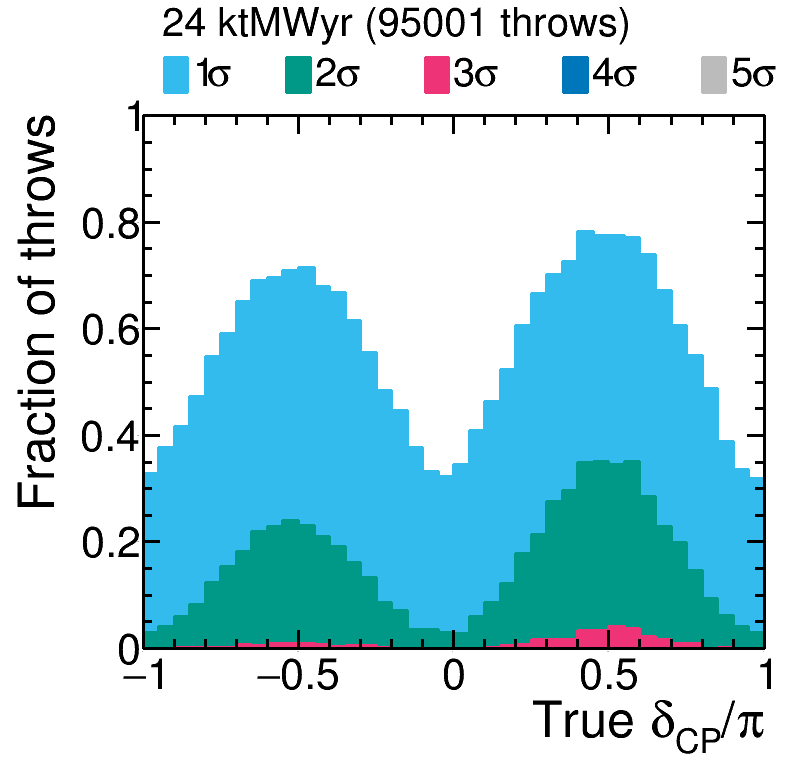
\includegraphics[width=0.33\linewidth]{cpv_throws_24ktMWyr_NH_th13.png}}
  \subfloat[66 kt-MW-yr] {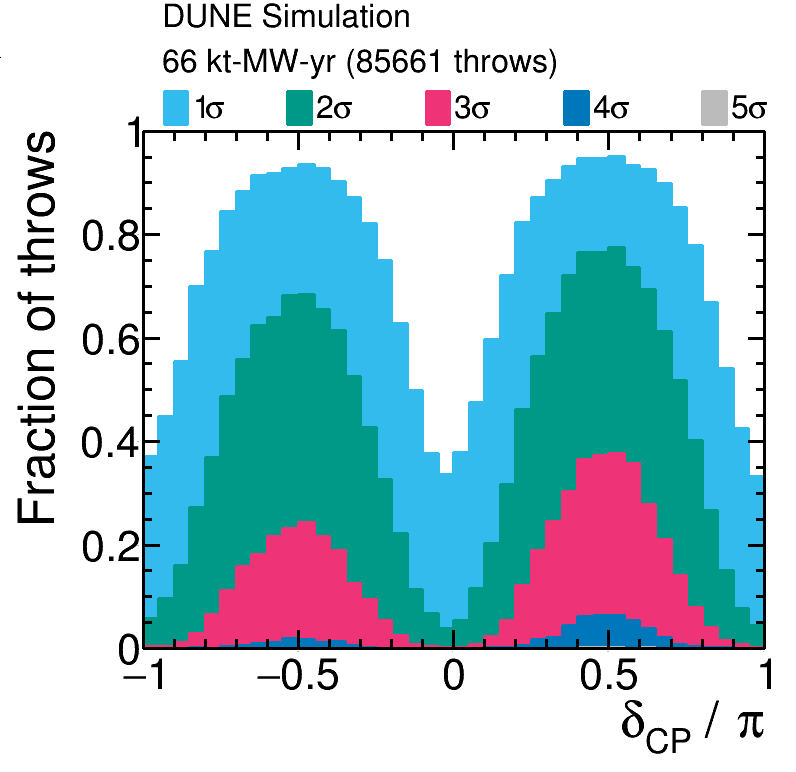
\includegraphics[width=0.33\linewidth]{cpv_throws_66ktMWyr_NH_th13.png}}
  \subfloat[100 kt-MW-yr]{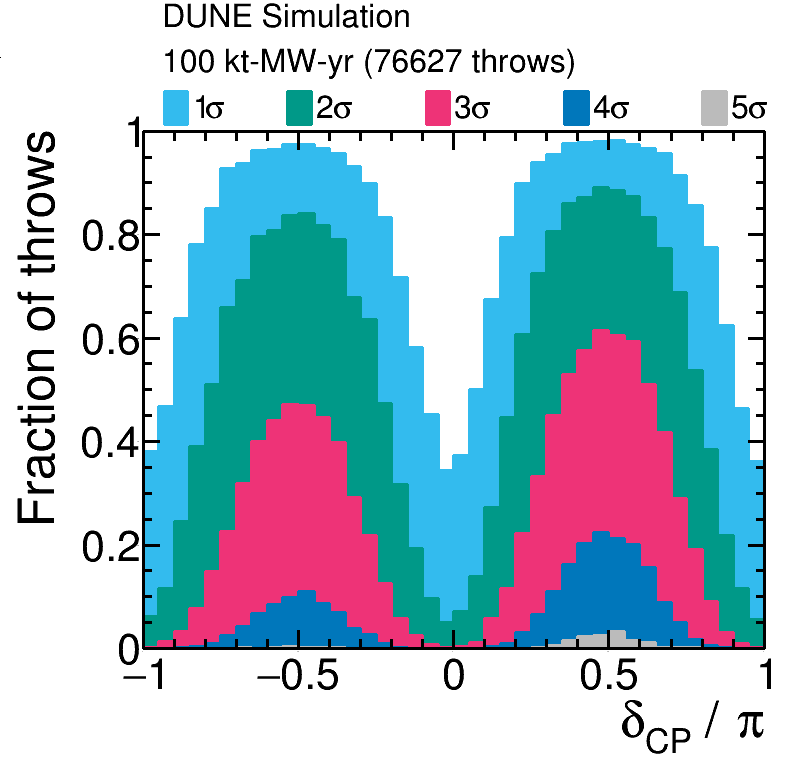
\includegraphics[width=0.33\linewidth]{cpv_throws_100ktMWyr_NH_th13.png}}\\
  \subfloat[150 kt-MW-yr]{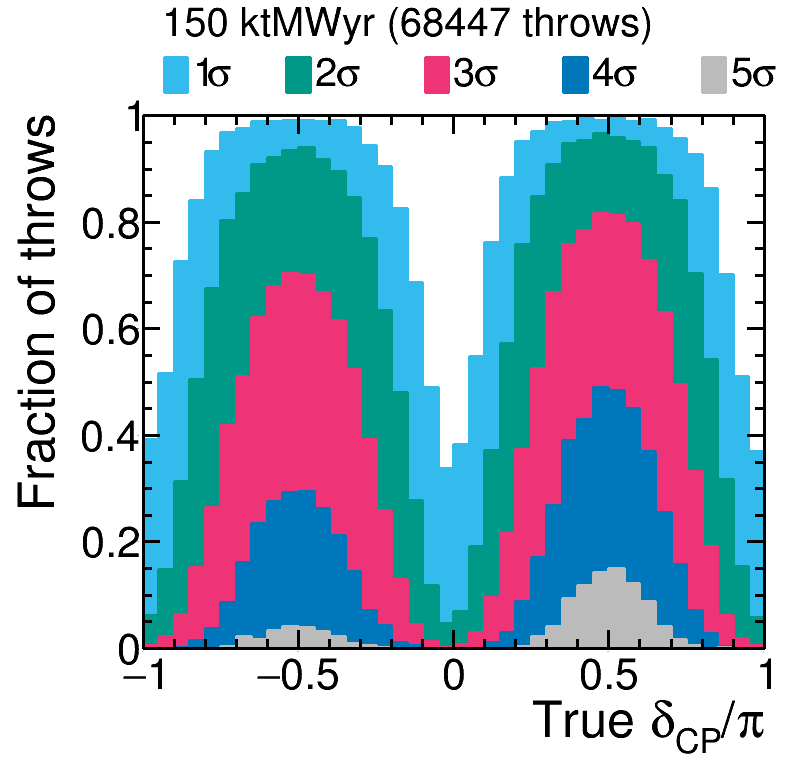
\includegraphics[width=0.33\linewidth]{cpv_throws_150ktMWyr_NH_th13.png}}
  \subfloat[197 kt-MW-yr]{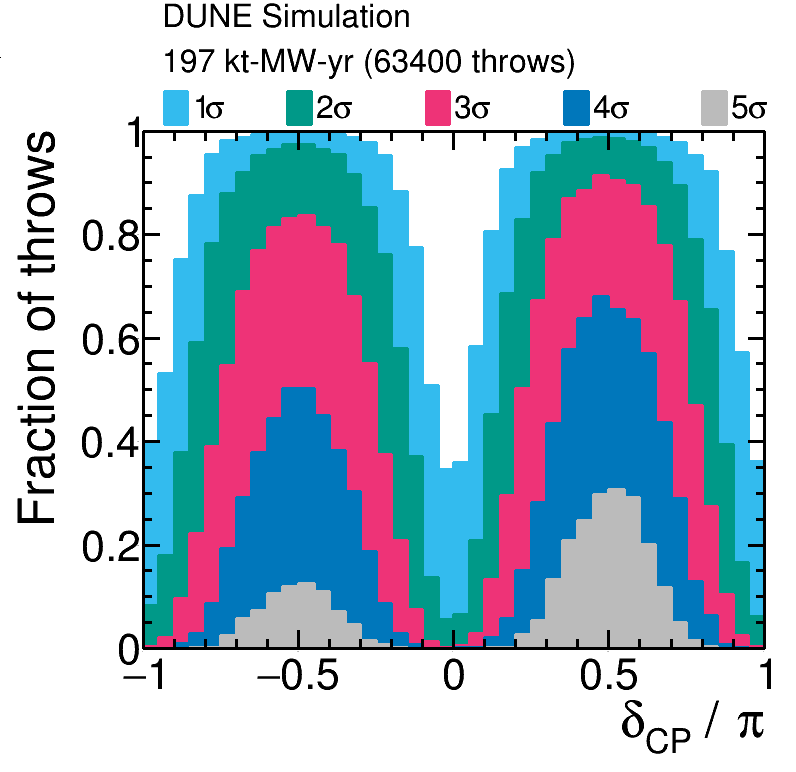
\includegraphics[width=0.33\linewidth]{cpv_throws_197ktMWyr_NH_th13.png}}
  \subfloat[334 kt-MW-yr]{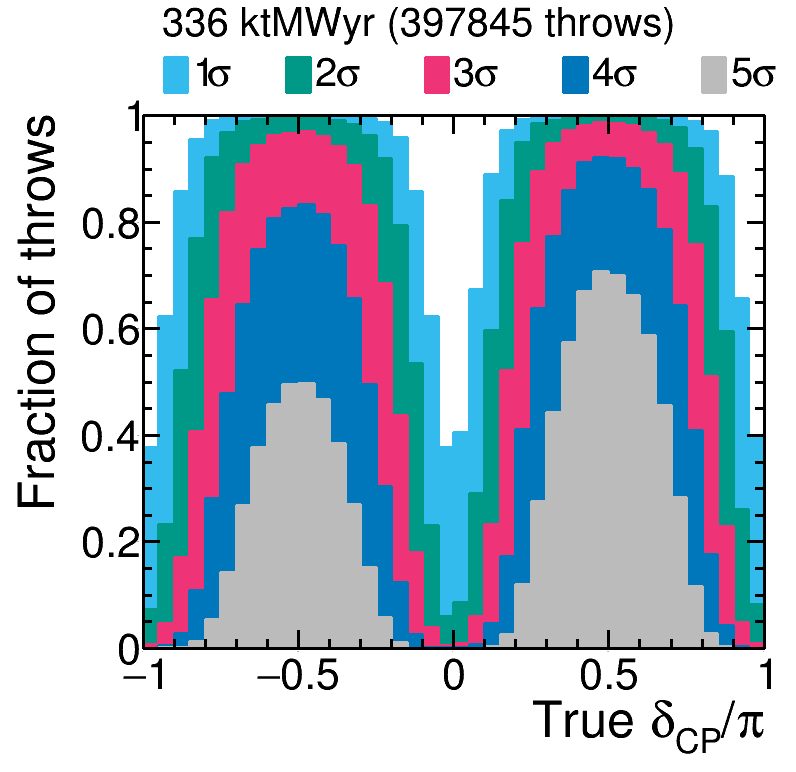
\includegraphics[width=0.33\linewidth]{cpv_throws_334ktMWyr_NH_th13.png}}
  \caption{Fraction of throws for which the significance of DUNE's CP-violation test ($\deltacp \neq \{0,\pm\pi\}$) exceeds 1--5$\sigma$, as a function of the true value of \deltacp. Shown for NO, for a number of different exposures. The number of throws used to make each figure is also shown.}
  \label{fig:cpv_over_time}
\end{figure*}
\begin{figure*}[htbp]
  \centering
  \subfloat[$\deltacp = -\pi/2$]     {\includegraphics[width=0.8\columnwidth]{{fraction_throws_vs_exp_dcp-0.5}.pdf}}
  \subfloat[50\% of \deltacp values] {\includegraphics[width=0.8\columnwidth]{{fraction_throws_vs_exp_dcprange_0.5}.pdf}}
  \caption{Fraction of throws for which the significance of DUNE's CP-violation test ($\deltacp \neq \{0,\pm\pi\}$) exceeds 1--5$\sigma$, both assuming $\deltacp = -\pi/2$, and for 50\% of \deltacp values, shown as a function of exposure, for NO.}
  \label{fig:cpv_vs_exp}
\end{figure*}

Calculating \dchisqcrit values above 3$\sigma$ using the FC method is challenging due to the large number of throws to explore the tails of the \dchisqFC distribution and prohibitive computational cost. In Figure~\ref{fig:cpv_over_time}, the fraction of throws that exceed 1--5$\sigma$ significance, calculated only with the constant-\dchisq method are shown in order to explore DUNE's sensitivity at higher significance levels. We note that all the caveats described above relating to the constant-\dchisq method still apply. Figure~\ref{fig:cpv_over_time} shows that although the median significance to CPV does not exceed 5$\sigma$ until $\sim$334 kt-MW-yr, there are significant fractions of throws at lower exposures which reach $5\sigma$ significance. Figure~\ref{fig:cpv_vs_exp} shows the fraction of throws which exceed different significance thresholds at the maximal CP-violating value of $\deltacp = -\pi/2$, and for 50\% of all \deltacp values, as a function of exposure. Note that by $\sim$200 kt-MW-yr, where the median significance for 50\% of the \deltacp range is greater than 3$\sigma$, the sensitivity at $\deltacp = -\pi/2$ exceeds 4$\sigma$.

\FloatBarrier
